% !TEX root = ../notes_template.tex
\chapter*{Introduction}
\addcontentsline{toc}{chapter}{Introduction}
\minitoc

This chapter introduces basic concepts for knowing and applying clinical physiology in physical therapy practice. First we consider what we mean by clinical physiology. Second we make sure all readers have the same understanding of the basic concepts of physiology. Along the way we introduce some of the broader aspects of the approach we are taking related to clinical epistemology and Unifying Systems Theory. Clinical epistemology is bound to the use of models to summarize, test and apply clinical knowledge. Unifying Systems Theory keeps us focused on the muscle fiber act of tensioning, and organizes our presentation of the quality attributes of that act such as fidelity, efficacy and integrity, and the ubiquity of fractal recursion in physiological systems. 

\vspace{5mm}

\textbf{Objectives include:}
\begin{enumerate}
    \item Explain a muscle centered approach to clinical physiology for the practice of physical therapy
    \item Provide an example of a model that is useful in physical therapy practice.
    \item Explain the basic concepts of physiology
    \item Explain how whole system function and capacity relates to multi system function and capacity. 
    \item Provide an example of how each basic concept of physiology applies to the analysis of patient/client problems.
    \item Explain the hierarchy of adaptation and adaptability from genetic, epigenetic, anatomic, physiologic, behavioral and cultural and its relevance in physiological adaptation.
    \item Explain how the International Classification of Function (ICF) clinical physiology relates to the hierarchy of adaptation and muscle centered approach..
\end{enumerate}

\subsection{A note about objectives}

Each chapter has objectives. They include specific behavioral terms related to the expectation for the objective. There is an ordered relationship between the behavioral terms that represents increasing and nested expectations. To define is to understand the words being used, to know what they represent. Whether you can define something can be tested with a straightforward question such as identifying the correct definition from a set of definitions; whether you can write the definition; respond true or false to a proposed definition for a term; or identify the correct term from a set of terms when presented with a definition. To explain something goes beyond defining. It also implies that you can define the required terms. To explain\footnotemark{}\footnotetext{Explain is the act associated with understanding. If you understand something you can explain it. Objectives are typically written as acts - what the person learning can do if they have achieved the objective. Since understanding is observed as an act of explaining, we will use the objective "explain" when there is something you must "understand". How do you demonstrate that you understand? You explain whatever it is that you understand.} you need to simultaneously hold a set of definitions together including how they relate to one another. You can explain a model by demonstrating that you know all the definitions involved, and describe how they relate to one another, and can communicate that explanation. Whether you can explain something can be tested by asking about several aspects of what you are to explain or asking you to infer which part is missing; or by asking about one part and asking you to infer the other part. The point is, to explain goes beyond defining and has an expectation of definition. But to define does not require you to explain. To evaluate something requires you to make judgements and to infer beyond the thing you are asked to evaluate. To evaluate implies that you can define and explain the thing (or concept) you are asked to evaluate. Being tested for whether you can evaluate can include asking you to infer to or from something that has not been directly covered or discussed, going beyond the thing (or concept)\footnotemark{}\footnotetext{By a "thing" we intend a particular thing, perhaps a particular object, whereas by a "concept" we intend a universal that will contain many particulars. For example, there is a muscle fiber as a thing, meaning this particular muscle fiber and there is the concept of muscle fiber, meaning anything that has the properties of being a muscle fiber, hence universal and conceptual. This idea of the particular (concrete) and the universal (abstract) is an important concept in and of itself for your practice as physical therapists. You have both a particular patient, perhaps Sean, and you have universal patient, perhaps everyone with heart failure.} you are asked to evaluate to consider its implications in different situations. Providing an example is an objective based on a specific task and is considered a form of asking you to evaluate since it goes beyond a particular thing (or concept) to a totally new thing (or concept). Asking you to provide an example of a model requires you to know the concept of a model well enough that you can use your background knowledge to come up with something you're already familiar with that fits what know about models. That level of knowledge requires you to at least be able to evaluate a model because you have essentially evaluated your background knowledge and determined that it is a model. The chapter objective above that asks you to provide an example of a model that is useful to physical therapy practice assumes you will be able to define, explain and evaluate the concept of a model, and that you have background knowledge about physical therapy practice that you can use to evaluate models used in practice to consider what those models are and whether they are useful. 

\section{Clinical Physiology}

Physiology is a foundational science for physical therapy. Clinical physiology focuses on physiology relevant to understand health and "un" health (injury, illness, disorder, dysfunction, disequilibrium). This is a clinical physiology text for physical therapists. Since physical therapists are movement specialists, and since the physiology of muscles is integral to the movement system, our approach to clinical physiology is a muscle centered approach.  A muscle fiber\footnotemark{}\footnotetext{Muscle fibers are muscle cells, and muscle cells are muscle fibers. We do our best throughout the book to refer to muscle fibers, but if we refer to a muscle cell please know that this equates to saying muscle fiber. Similarly, when we talk about the general biological properties of cells, please know that these properties are true for muscle fibers} is a system, and muscle fibers are the structural unit of muscle. A system is whole and acts (works towards a common objective). A system has agency (ability to act to satisfy values). 

%Correct (fidelity), complete (integrity), concise (efficacy)

The act of a muscle fiber is tensioning (act of creating tension). As a system that acts by creating tension muscles are correct, complete and concise. A muscle fiber correctly acts to create tension, it is complete (has what it needs for that act), and it is concise in creating tension. A muscle fiber interacts with other systems and is supported in order to satisfy its act. Much of clinical physiology for a physical therapist considers the act of muscle tensioning, what and how a muscle fiber interacts with other systems, and what support is required for the muscle fiber to act.

When a muscle fiber acts to create tension it attains and sustains tension for movement. To satisfy this act muscle fibers interact and are supported. Therefore interactions and support are an important part of the book. Muscles get a lot of their support from the the extra cellular fluid (ECF), and maintain their ability to create tension through cellular and structural integrity.

Clinical physiology for physical therapy with considers the three interactions depicted in Figure \ref{fig:muscle_centered_approach}.  The first interaction considers the relationship between muscle cells and movement, second between movement and extra cellular fluid, and third between extra cellular fluid and muscle cells. These interactions are all support relationships. The first is an undeniable part of the movement specialist’s domain of knowledge and an area that most physical therapy students have little problem understanding how important it is for them to understand. The second and third relationship are less obvious and deserve additional explanation. The following sections explain these supporting interactions.

\begin{figure}[!ht]
    \centering
    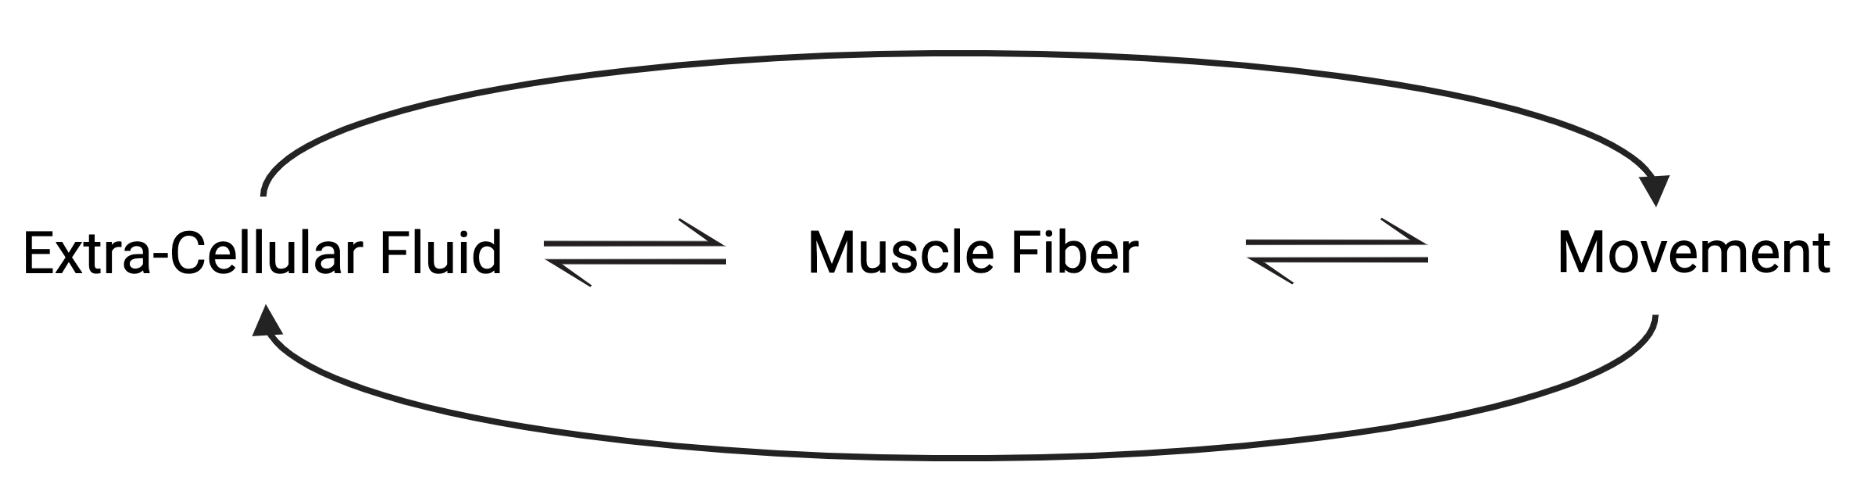
\includegraphics[width=1\linewidth]{./figure/muscle_centered_approach.png}
    \caption{A Muscle Centered Approach \footnotesize{(Created with BioRender.com)}}
    \label{fig:muscle_centered_approach}
\end{figure}

\subsection{Muscle Fibers and Movement}

Muscle fibers are necessary but not sufficient causes for human movements. Muscles cause movement by creating tension. Active and passive tension and a whole host of details are being skipped here (such as parts, capabilities, roles and interactions) combine to create movement.

Muscle fibers create tension but cannot do this alone.  First, muscle fibers must come together as a muscle and combine their ability to create tension in order to create movement. They create tension with interaction to attachments, mostly, to bones\footnotemark{}\footnotetext{Mostly to bones because sometimes muscles attach to something other than bones such as the eye muscles or facial muscles that attach to skin to create facial expressions, or muscles that attach to themselves.} that form joints that are capable of movement. The process of coming together, and creating tension and transmitting tension to bones is covered in the next two chapters (Fundamentals and Tension). Other aspects of movement such as the mechanics and kinematics of the musculoskeletal system, or the coordination, control and learning of the neuromotor and behavioral systems, are not covered in this book. To create tension muscles need to possess the capabilities of being excited (provoked into creating active tension), being regulated to create the right amount of tension, and converting energy. Excitation, Regulation and Energetics are covered in Part II, Muscle Fidelity and Efficacy. 

\subsubsection{Muscle Fidelity \& Efficacy}

Muscle Fidelity focuses on attaining tension. The parts and capabilities of muscle fiber that allow it to attain tension when needed. Metrics of fidelity assess how well tension is attained such as measures of force.

Muscle Efficacy focuses on sustaining and transforming tension. How well does muscle sustain tension once attained, and how well does it transform tension to its intended use, typically in interaction with something outside of or beyond muscle itself. Metrics of efficacy assess how effectively (including efficiently) muscle fulfils its purpose and includes whether the muscle can sustain (continue to generate a tension) and persevere (continue to repeat the process of sustaining tension). Efficacy metrics consider time along with force, commonly referred to as endurance, or force and energetics (efficiency). 

\subsection{Extra-Cellular Fluid and Muscle Fibers}

The capability to create tension requires support. Support is received from the surroundings of the muscle fiber, the extra cellular fluid (ECF). ECF is supported and tightly regulated through the activity of several physiological systems. In this sense, as depicted in Figure \ref{fig:muscle_centered_approach}, the ECF causes (in a supportive role) muscle tension.\footnotemark{}\footnotetext{It is admittedly much more complicated than this and the use of the term causes can be challenged, but the assertion is that without the proper ECF muscle active tension cannot occur. It is true that muscle passive tension can occur with a passive stretch of the muscle but such a passive stretch is typically the product of another system putting energy into the muscle to create the passive stretch and that other system putting energy into the muscle often relies in some way on ECF.} When a muscle fiber creates tension it utilizes and exchanges resources with the ECF, thus muscle cells thus rely on and contribute to ECF. These systems that refresh and regulate the ECF are the focus Part III, Muscle Support and include the circulatory, renal, pulmonary, gastrointestinal, metabolic (liver and pancreas), and neuroendocrine systems and physical laws upon which physiological function is based (diffusion and osmosis, mass balance, flow based on gradients to name a few).

\subsection{Movement and Extra-Cellular Fluid}

The ECF contains and sustains the correct materials for supporting and supplying muscle fibers. The ECF and all the systems that support it are also supported by the ECF. The ultimate source of materials in the ECF is movement (Figure \ref{fig:muscle_centered_approach}). It may be the movement of the heart, the movement of the arterioles that regulate blood flow, the movement of the breathing muscles that move air into and out of the lungs, the movement of limbs to get food and water, the movement of the jaw and esophagus and gastric tube to digest and move food and water for absorption, the movement of the colon for waste products. These have all been examples of movements caused by muscle tension in support of the ECF that is ultimately supporting the muscle fibers causing the muscle tension.


\subsection{Muscle Integrity}
Muscle Integrity focuses on muscle fibers being muscle fibers, capable of generating tension. Muscle fibers exist to execute the act of generating tension so integrity is about the parts and capabilities that make a muscle fiber a muscle fiber. Muscle Integrity considers both ECF in support of, and movement influencing, muscle fibers. ECF supports the long term act of creating muscle tension by providing the necessary resources for the muscle to maintain its integrity (it continues to be a muscle and therefore to be able to do the act of creating tension). Movement is also involved (the arrow from movement to muscle in Figure \ref{fig:muscle_centered_approach}) because movement, as you probably know, provides (or does not provide) a stimulus for the muscle fiber. Muscle cells create movement and movement creates stress and strain on muscle fibers that act as triggers for myostasis (muscle fibers continue to be, which we will call isotrophy) or to grow (hypertrophy) and when not needed to reduce their need for resources (atrophy). Isotrophy, hypertrophy and atrophy occur on a spectrum covered in Part III Muscle Integrity. Muscle Integrity includes the cellular activity occurring within muscle fibers, and is supported by the ECF and stimulated by movement.

Metrics of Muscle Integrity include the ability to continue to do what a muscle cell does (persevere) which occurs through maintaining the various parts, capabilities and interactions. A measurement of integrity could be the cross section area of a muscle, or the lean mass of muscle, as indicators of how well the muscle (as a muscle collection of muscle fibers) is being maintained.

\subsubsection{Fractal Recursion}
The cycle depicted in Figure \ref{fig:muscle_centered_approach}, ECF causes muscle tension causes movement causes ECF, and so on, is called fractal recursion. There are many examples of fractal recursion in physiology. A muscle fiber is supported by the ECF, which is supported by the micro-circulation, which is supported by blood flow, which is supported by blood volume, which is supported by drinking, which is supported by the movements of acquiring fluid to drink, which is supported by muscles. There are numerous supported:supporting relationships nested within physiology.

%An example of fractal recursion is the Supported/Supporting pattern. The pattern repeats at any scale up or down. Perhaps in this example, start with Tensioning (Supported) / Muscle (supporting). Then we take Muscle-integrity (Supported) / ECF (Supporting). The other concept in play here is the notion of federation toward unification. So Movement as an example (Unifying objective) can be supported at the first level by bone (Counterpoising), muscle (Tensioning), tendon (Anchoring) and cartilage (Bearing). Using fractal recursion to differentiate further, muscle tensioning (Supported) is the unifying objective and ECF (Supporting) facilitates the sustaining acts of "Fueling" and "Wasting".

\subsection{Models}

Figure \ref{fig:muscle_centered_approach} constitutes a model. Models are simplified abstractions of reality. This model does not include all the details. It is not supposed to include all the details. If it included all the details it would be overwhelming. Hashing out just some of the detail requires the rest of this book. Hashing out more of the details includes most of your education. Hashing out all of the details is not currently possible and requires more than one lifetime.\footnotemark{}\footnotetext{The lifetime of many scientists has already been spent on hashing out the details that we currently know. Some may say that all the details is computationally intractable considering the depth of mechanisms at the molecular level.} Hashing out the details we continue to create and consider additional models, over and over again, models of models of models of models (fractal recursion) as we successively approximate something useful to understand and knowledge to base practice.

There are numerous models throughout this book. With each model we consider a quote by George Box: “All models are wrong some models are useful.” The muscle centered approach is our first step. Three variables and interrelationships provide a model of clinical physiology as a guide to reasoning for physical therapists in the context of injuries, conditions, and diseases. This is a useful model. There are certainly going to be situations that don’t fit the model since not all details are contained in the model. But for the task of learning clinical physiology to practice physical therapy, it's useful. 

\paragraph{More about models}

We build models in order to summarize, test and apply our knowledge \cite{collins_synthesis_2018}. Models come in many forms - graphic, causal, logical, mathematical, computational, even stories are examples of models. There are many models about muscles utilized to summarize, test and apply knowledge about muscles. For example, the sliding filament theory is a model about how muscles develop active tension featured in Chapter \ref{chp:tension} on Tension. The sliding filament theory was developed based on striated appearance (overlapping filaments) and the observation that length of muscle influenced the overlap of striations and was related to how much tension could generated when excited (length - tension relationship). The inference proceeds, if these filaments slide past each other to generate tension then overlap changes with length and should influence how much tension can be generated. So the sliding filament model proposed the length-tension relationship as a hypothesis. It then received experimental support when the length - tension relationship was observed. The muscle acted as expected if the sliding filament model was true. Based on the sliding filament model, and based on the length - tension curve (behavior predicted by the model), there are joint positions to test a muscles ability to generate maximum active tension (force). This model of muscle, sliding filaments and length - tension, is applied in practice. It is a model of muscle that is true for all striated muscle (including cardiac muscle, striated but differentiated from skeletal muscle).

This book and your education and practice is full of models that summarize, test and apply knowledge of muscles and physiological systems that support them. Just remember, models are abstractions of reality, not reality. "All models are wrong, but some models are useful" (George Box). Compared to reality all models are limited. Always ask We must whether the model being applied is useful - useful to test what we think we know, useful to summarize what we know, and useful to utilize what we know.

\subsection{Clinical Physiology Summary}

Clinical physiology from a muscle centered approach starts with a simple model. Based on this model if a PT considers muscles as a cause of movement but doesn't consider the factors that influence the ECF that is critical to the excitation, regulation, energetics\footnotemark{}\footnotetext{The convention we will utilize is that word "energetic" is an adjective, something is energetic, marked by vigor or effect, related to energy. However, adding an 's' to the end of energetic, energetics changes it to a verb, the process of converting energy and should not be confused as a plural form of the adjective energetic.} and integrity of the muscle fibers then they are ignoring a critical component of the supported:supporting relationship. If a PT considers how the ECF influences muscle fibers and thus movement and does not consider how continued movement influences the ECF they may miss the opportunity to stop repeated hospital admissions.\footnotemark{}\footnotetext{Such as readmissions due to repeated breakdowns in a person that goes home, cannot move enough to sustain hydration or nutrition or ventilation and returns to the hospital dehydrated, malnourished and with pneumonia \cite{collins_heart_2015}} Considering these three supported:supporting fractal recursive variables is a first step to thinking about clinical physiology with a muscle centered approach for the purpose of practicing physical therapy.

\section{Basic Concepts of  Physiology}

The Basic Concepts of Physiology provide a unifying framework that we apply throughout the book. They are a summary of the pre-requisites for reading this book, which is aimed at physical therapy students (graduate level) who are expected to have already be familiar with the basics of physical, chemical and biological sciences. In this section we consider each of the basic concepts provide insights of how they are useful to the physical therapist. We consider how the basic concepts of physiology are applied to the analysis of patient/client problems and are a foundation for understanding altered physiological states (pathophysiology).

\subsection{Causality}
Living organisms have causal mechanisms whose functions are explainable by a description of the cause-effect relationships that are present. Much debate exists about what constitutes a causal mechanism and relationship, and identifying as well as specifying causal relationships and models (to understand mechanisms) are an important part of physical therapy practice \cite{collins_synthesis_2018}. Accepting that these causal mechanisms are explainable is a philosophical assumption, just because many cause-effect relationships are explainable we still must deal with what is called the problem of induction. We attempt to solve, or at least manage, the problem of induction through rigorous manipulation and observation (experiment) or systematic observations (epidemiology) and subjecting these observations to statistical inference. Regardless of of what we know, or can know, about causal relationships and mechanisms based on what we observe, is the assumption that underlying any effect we observe there is a cause, or a set of inter-related causes. This is an essential aspect of causality as a basic concept of physiology and we will be applying this basic concept every step of the way.
\paragraph{}
Causality is applied to the analysis of patient/client problems through the very fact that if we observe an effect we infer some underlying cause. If there is an alteration in blood pressure, glucose or sodium we infer something is the cause of those alterations. Inference from effects to causes is called abduction, and when there are multiple possible causes from a set of effects, is called inference to the best explanation. The statistical inference used to calculate the probabilities of inferences from causes to effects is called Bayesian inference and it is the foundation of any diagnostic process. 
\paragraph{}
Muscles generate tension. Tension is an effect. Part I considers the causes of that tension. If muscles generate too much or too little tension (an effect that is noticed as muscle stiffness or muscle weakness) then we consider the causes of the tension and what may be wrong, why are they not currently causing the right amount of tension? 

\subsection{Cells}

\subsubsection{Cell Theory}

Cell Theory states that all cells making up an organism have the same DNA. Cells are considered the basic unit of life. All of the specialized functions we cover in this book are based on differentiation and the subsequence specialization of cells throughout the body.   
\paragraph{}
Cell Theory is applied to the analysis of patient/client problems through the observation of the health and well being of cells as an indication of whether there are problems, first with the cell, and second as a possible abnormal cause. For example, any cells that divide at a rapid rate (which itself is the result of DNA expression specific to the specialization of the cell), such as skin cells, have a greater chance of DNA mutation during cell division. A DNA mutation during skin cell division can result in a variety of benign or malignant cancerous cells that appear on the surface of the skin. The presence of a mole, particularly one that is not circular or has rough edges, is a possible sign of altered DNA of those cells creating cancerous cells. A benefit to having a high rate of cell division is ability of these cells to replaced dead or damaged cells resulting in faster healing and complete repair as opposed to an adaptive repair.

\paragraph{}
Extending the concept of the rate of cell division further is the general principle that areas of the body with lower rates of cell division (chondrocytes, cells that spawn cartilagenous material), or sometimes so low to be observably absent (some nervous system cells), are known to have slower or absent rates of healing and repair. When we consider osteoarthritis as a "wear and tear" of the joints we are saying that the rate of wear and tear exceeds the rate of healing and repair, which are determined in large part by the rate of cellular division in those specialized cells. Whether a supplement such as chondroiten (a molecule found in cartilage) helps treat the symptoms of osteoarthritis is dependent on whether the cause of the imbalance between damage and repair has something to do with not having enough chondroiten, or whether chondroiten does not just provide material, but is coupled in some way with increasing the repair process.
 
\subsubsection{Cell Membrane}

The boundary of a cell is delimited by a semi permeable plasma membrane, the cell membrane. In a muscle fiber it is the sarcolemma. The sarcolemma is a complex structure that determines what substances enter or leave the muscle fiber. It is the boundary between the inside of the cell (cytoplasm, for a muscle fiber the sarcoplasm) and the outside of the cell (ECF). The sarcolemma is essential for cell signaling, transport and other processes. The proteins (receptors, channels, pumps) embedded in the sarcolemma influence how permeable the membrane is to certain substances, and thus how quickly those substances can enter (or exit) the cell. Many of the adaptations to muscle fibers to exercise training are related to changes in the proteins of the sarcolemma that allow certain muscle acts to occur more rapidly - such as excitation for example. To increase the rate of excitation the sarcolemma can include additional sodium/potassium pumps, more sodium and potassium channels that allow faster excitation cycling (discussed in much more detail in Chapter \ref{chp:excitation} on Muscle Excitation).

\paragraph{}
The cell membrane is applied to the analysis of patient/client problems in a rather fundamental way. Whether a cell is a cell includes whether it has a boundary. If damage to the cell membrane is complete, the cell no longer exists, it is dead. The assessment of cardiac cell death (infarction) includes whether certain proteins that are found in the cardiac muscle are in the blood. The reasoning is that for those proteins to be in the blood, they had to escape the cardiac muscle and that can only happen if the cell membrane is irreversibly damaged, and if the cell membrane is irreversibly damaged then the cell is dead. Therefore, if there is Troponin I or T in the blood, or Creatine Kinase - Myocardial Band (CK-MB) in the blood, then some sort of cardiac muscle fiber infarct has likely occurred.

\subsubsection{Cell-Cell Communication}

This may seem like a nit but what if you inverted the order/emphasis of this statement. The expression of a function by a federating (multi-cellular organism) requires the ability to coordinate individual action typically utilizing the most concise means. Just a thought.

The function of any multi-cellular organism requires the ability to coordinate individual action typically using the most concise means. This can be achieved by cells passing information to one another through "cell-cell communication". These communication processes include endocrine (hormones delivered system wide in the blood which alert all muscle fibers receiving blood flow that have a receptor within their sarcolemma) and neural signaling (which tends to more specifically target particular muscle fibers). 

\paragraph{}
Cell-cell communication is applied to the analysis of patient/client problems in any situation where endocrine or nervous system interactions with the cells may be abnormal. The release of insulin signals to cells that they should increase their glucose uptake. If cell-cell communication is impaired, as with Type II Diabetes, and the insulin receptors on the cell do not adequately receive that communication then cells will not uptake more glucose in response to insulin and blood glucose values will increase. One possible cause of an elevated blood glucose is a problem with cell-cell communication of the insulin receptors not responding to insulin. 

\subsection{Genes to proteins}
Genes (DNA) code for the synthesis of proteins (muscle filaments and enzymes are proteins). This is not all the genome\footnotemark{}\footnotetext{All the genes together} or the epigenome\footnotemark{}\footnotetext{Above the genome, the meta genome}, does, but it is an important part of muscle cell differentiation, specialization and myostasis. The genes in a particular cell that are expressed determine the functions of that cell (i.e. make it a muscle fiber and not, say, a liver cell), and additionally can make it a particular type of muscle fiber (i.e. a fast or slow twitching muscle fiber). Genes to proteins are an important component of Part III: Muscle Integrity.

\paragraph{}
Genes to proteins is applied to the analysis of patient/client problems whenever we consider the impact of cancer (mutations in DNA during division that then influence the proteins being created) on cellular function. Genes to proteins is also the fundamental process by which muscle fibers are maintained (myostasis - isotrophy, staying the same) or adapt (myostasis - hypertrophy or atrophy). Mechanisms generating tension in the muscle fiber are dependent on proteins, and the proteins are produced during the translation and transcription of DNA. 

\subsection{Energy}
The life of the organism requires the constant expenditure of energy. The acquisition, transformation, and transportation of energy are essential functions. Experimental approaches to understand muscle are focused on muscle fibers as energy conversion machines, taking chemical energy and converting it into mechanical energy \cite{woledge_energetic_1985}. 
The earliest of these studies measured work and heat based on the physical law of the conservation of energy. Energy is neither created or destroyed. Energy is transformed from one form to another. When a muscle fiber breaks down adenosine triphosphate (ATP) to generate tension, as discussed in Chapter \ref{chp:energetics} on Muscle Energetics), the energy of that chemical bond is transformed to mechanical work (force x distance) or as heat \cite{hill_heat_1938}.

\paragraph{}
Energy is applied to the analysis of patient/client problems since life is dependent on the constant expenditure of energy, and therefore requires ongoing acquisition, transformation, and transportation. If muscle fibers lack the fidelity and efficacy to allow movements that enable the acquisition of energy (consumption of nutrients), then muscle will subsequently lack integrity (atrophy, loss of muscle mass) due to the organisms continual need to acquire energy. Muscle integrity is sacrificed in situations of malnutrition or starvation, even when that malnutrition or starvation is caused by the inability to move. 

\subsection{Mass Balance}
The quantity of ”stuff” in any system, or in a compartment of a system, is determined by the inputs into the system and the outputs from that system or compartment. This concept is based on the law of conversation of mass. When someone consumes 50 grams of carbohydrate (CHO) those 50 grams are then part of them and will be processed (digested, metabolized and either eliminated, stored or otherwise utilized). 

\paragraph{}
Mass Balance is applied to the analysis of patient/client problems any time we consider the amount of some physiological variable, and this is ubiquitous in practice. Blood volume of all of the components that make up blood volume must be there in just the right mass balance for the ECF to have just the right mass balance for the muscle fibers to have just the right mass balance. When blood work is performed in a lab for a patient it is a general check on whether mass balance is being maintained on a whole host of components of blood volume.

\subsection{Flow Down Gradients}
The transport of “stuff” (ions, molecules, nutrients, blood, and gas) is a central process at all levels of organization in the organism, and a simple model (Ohm’s Law) describes such transport. 

Ohm's Law describes the relationship between current (flow of electricity), voltage and resistance:
\begin{equation} 
\label{ohms_eq}
Current = \frac{Voltage}{Resistance}
\caption{Ohm's Law}
\end{equation}

For fluid transport, such as blood through vessels and air through the airways we consider:
\begin{equation} 
\label{flow_eq}
Flow = \frac{Pressure}{Resistance}
\caption{Ohm's Law applied to Flow}
\end{equation}

For diffusion across membranes we consider:
\begin{equation} 
\label{diffusion_eq}
Diffusion = \frac{Concentration}{Resistance}
\caption{Ohm's Law applied to Diffusion}
\end{equation}

In all of these examples, which come up frequently through the book, current, flow and diffusion are proportional to the voltage, pressure or concentration gradient (numerator), and inversely proportional to the resistance (denominator). This is an essential concept. This model can be expanded for additional context and explanation. For example, considering the factors that influence resistance of blood flow (expanding the denominator) provides additional context and explanation for the regulation of cardiac output. 

\paragraph{}
Flow Down Gradients is applied to the analysis of patient/client problems any time we are considering pressure (blood pressure, oxygen partial pressure, etc) or concentrations (sodium concentration in the ECF). Disturbances in these pressures or concentrations fundamentally disturbs the flow that is necessary for normal physiological function.

\subsection{Homeostasis}
The internal environment of an organism is actively maintained constant by the feedback function of cells, tissues, and organs organized into primarily negative feedback systems.\\
Important points about homeostasis:
\begin{itemize}
    \item Not everything is regulated (i.e. heart rate)
    \item Homeostasis is not an on/off switch
    \item ”Relatively constant” – meaning there can be acceptable variation
    \item Set points can change
    \item There is a hierarchy of homeostatic regulation
\end{itemize}

The hierarchy of homeostatic regulation includes the fact that cells manage their internal environment (homeostasis), which includes taking and giving molecules and water to the ECF, the ECF is kept in homeostasis via exchange  with the blood volume (intra-vascular ECF) and homeostasis of the blood volume (water, cells, electrolytes, nutrients, etc) is exchanging with organ systems (lungs, liver, pancreas, gut). A simple graphic model of glucose homeostasis is shown in Figure \ref{fig:glucose_homeo} and shows the interactive relationship between glucose, glucagon and insulin.

\begin{figure}[!ht]
    \centering
    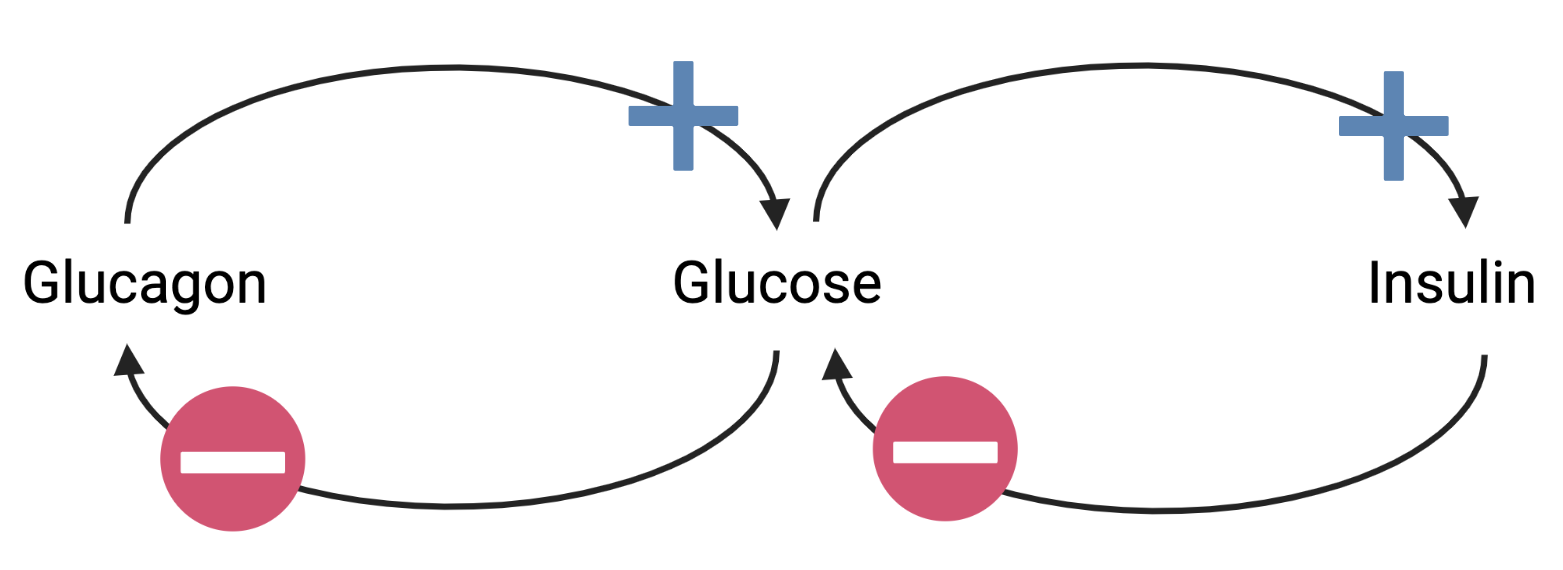
\includegraphics[width=1\linewidth]{./figure/glucose_homeo.png}
    \caption{Simple Model of Glucose Homeostasis that does not consider the organs or cellular mechanisms underlying the homeostatic relationship between the three components. In this system, glucose is being regulated. \footnotesize{(Created with BioRender.com)}}
    \label{fig:glucose_homeo}
\end{figure}

Figure \ref{fig:complete_glucose_homeo} A more complete model of glucose regulation starts by including the multiple paths by which glucose can be regulated and the role of metabolic organs such as the liver and the endocrine pancreas.

\begin{figure}[!ht]
    \centering
    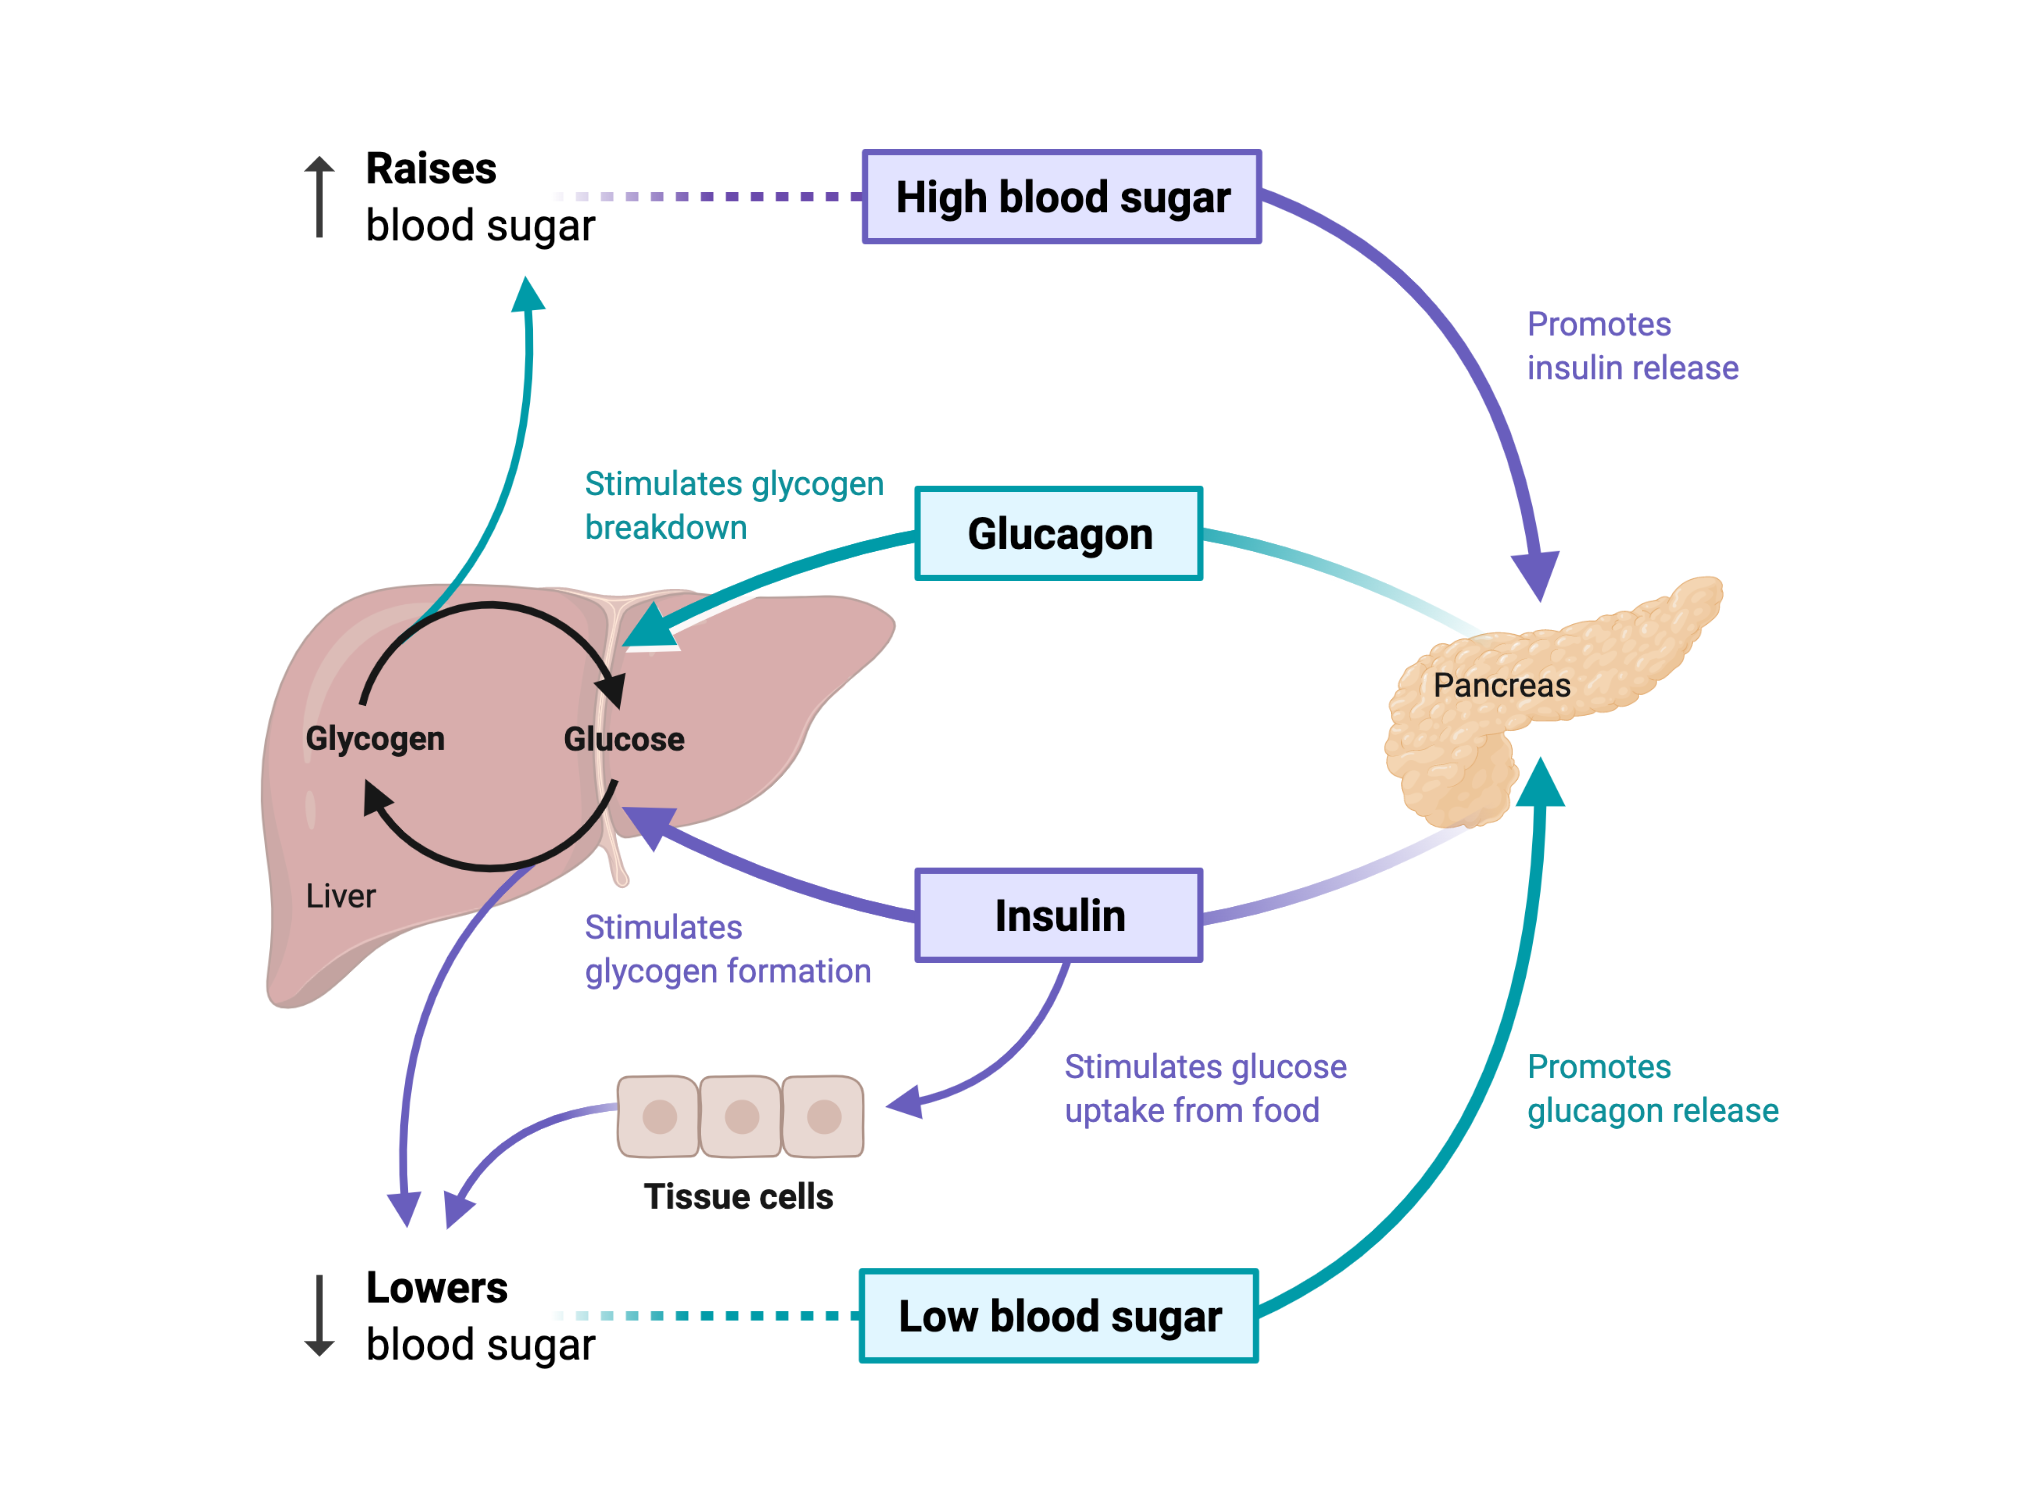
\includegraphics[width=1\linewidth]{./figure/complete_glucose_homeo.png}
    \caption{Model of Glucose Homeostasis that includes the organs involved in this homeostatic system \footnotesize{(Created with BioRender.com)}}
    \label{fig:complete_glucose_homeo}
\end{figure}

\paragraph{}
Homeostasis is routinely applied to the analysis of patient/client problems. Many diseases, conditions and syndromes, regardless of their underlying cause, results in some sort of disturbance to homeostasis; and thus any disturbance in homeostasis is ultimately analyzed for the possible causes.

\subsection{Interdependence}
Cells, tissues, organs, organ systems interact with one another (are dependent on the function of one another) to sustain life. Interdependence is includes nested and fractal recursive hierarchies of homeostatic regulation (supported:supporting relationships). The function and capacity of the "whole system" (the word for health comes from the word for whole) is related to the interdependent relationship between the parts, capabilities and attributes of each of the multiple systems acting together in supporting and supported roles. 

\paragraph{}
Interdependence is applied to the analysis of patient/client problems during the process of differential diagnosis. This process includes asking the "inference to the best explanation" question - "What are all the things that could cause this problem?" Given the interdependence of the whole system (the whole person), what contributes a list of potential causes for the observed effects?

\subsection{Structure - Function}
The function of a cell, tissue, or organ is determined by its form. Structure and function (from the molecular level to the organ system level) are intrinsically related to each other. Structure influences function (right now) and function influences structure (eventually). Much of Part II Muscle Fidelity and Efficacy is how structure influences structure right now; and Part III Muscle Integrity includes how function influences structure eventually (hypertrophy and atrophy).

\paragraph{}
Structure - Function is applied to the analysis of patient/client problems in the process of diagnosis of pathoanatomical conditions and also is the foundation for pathokinesiological interventions. If function is impaired, we consider the structure that may result in such an impaired function. For example, if there is an deviation in the gait pattern (function), we may consider the length of the hip flexors (structure impacts function). Also, if there is a functional movement deviation, prolonged sitting (function), we may teach corrective exercises to prevent future changes in structure (shortened hip flexors) that become dysfunctions (function impacts structure eventually).

\subsection{Hierarchy of Adaptation}

There is a hierarchy of adaptation and adaptability working within and around physiological systems. Adaptation refers to changes that occur to the system so that it optimizes fidelity, efficacy and integrity when completing its act. A muscle fiber act is creating tension. Adaptation refers to changes that occur in a muscle fiber to meet the needs of applying tension (fidelity), transforming the muscle fiber to meet the needs of applying tension in a more efficient way (efficacy), and changes to the muscle fiber that allow it to continue to be a muscle fiber (integrity). Adaptability refers to the ability to adapt. The hierarchy includes genetic, epigenetic, anatomic, physiologic, behavioral and cultural changes. Cultural changes being a mechanism of passing behavioral adaptation from one generation to another. This entire hierarchy is involved through the life span and has relevance to physiological adaptation. Very clearly all of those that are within connect directly to physiological adaptation (genetic, epigenetic, anatomic, physiologic). Behaviors are enabled by our physiology, but then also influence our physiology (our physiology allows us to eat sugar, and then our eating of sugar influences our physiology). And the culture around us gives rise to acceptable, and not acceptable, behaviors. 

\paragraph{International Classification of Function (ICF)}
Physical therapists incorporate the hierarchy of adaptation with the World Health Organization's International Classification of Function (ICF), see Figure \ref{fig:icf}. The ICF is a model that describes how physiological systems contribute (as body systems and functions) and interact with functioning (or dysfunction or impairments). The ICF model focuses on the bidirectional interactions between bodily functions (and structures), activities (movements and behaviors) and participation (behaviors and interactions). It also considers to health conditions that impact functions, activities and participation along with external and personal factors. 

\begin{figure}[!ht]
    \centering
    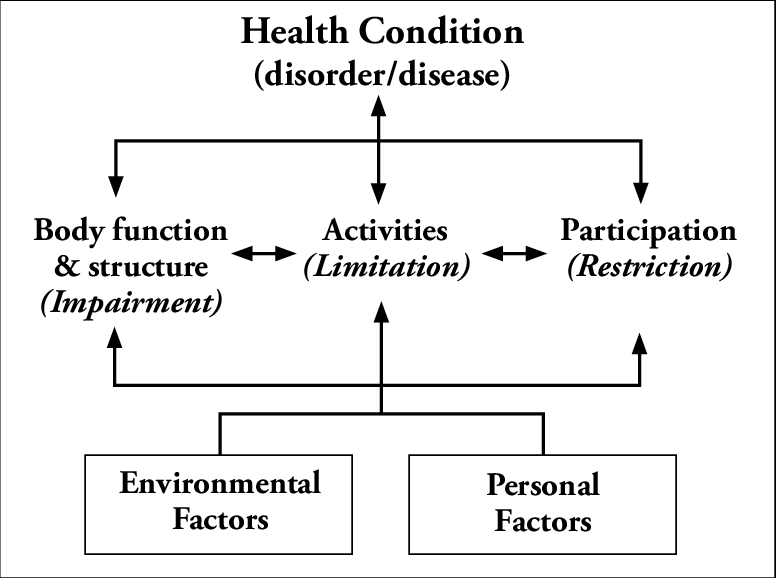
\includegraphics[width=1\linewidth]{./figure/ICF.png}
    \caption{International Classification of Function (ICF) \footnotesize{(Created with BioRender.com)}}
    \label{fig:icf}
\end{figure}

The ICF is a useful model for physical therapy practice. It is useful for understanding physiological interdependence, structure - function relationships, and the hierarchy of adaptation. The middle of the ICF is \textit{Activity}, which is primarily referring to movement, making the ICF a movement centered approach. The model considers what is necessary for movement, body structure and functions; and why we do movements, to participate. In this way the ICF overlaps with our muscle centered approach as depicted in Figure \ref{fig:muscle_centered_approach_icf}

\begin{figure}[!ht]
    \centering
    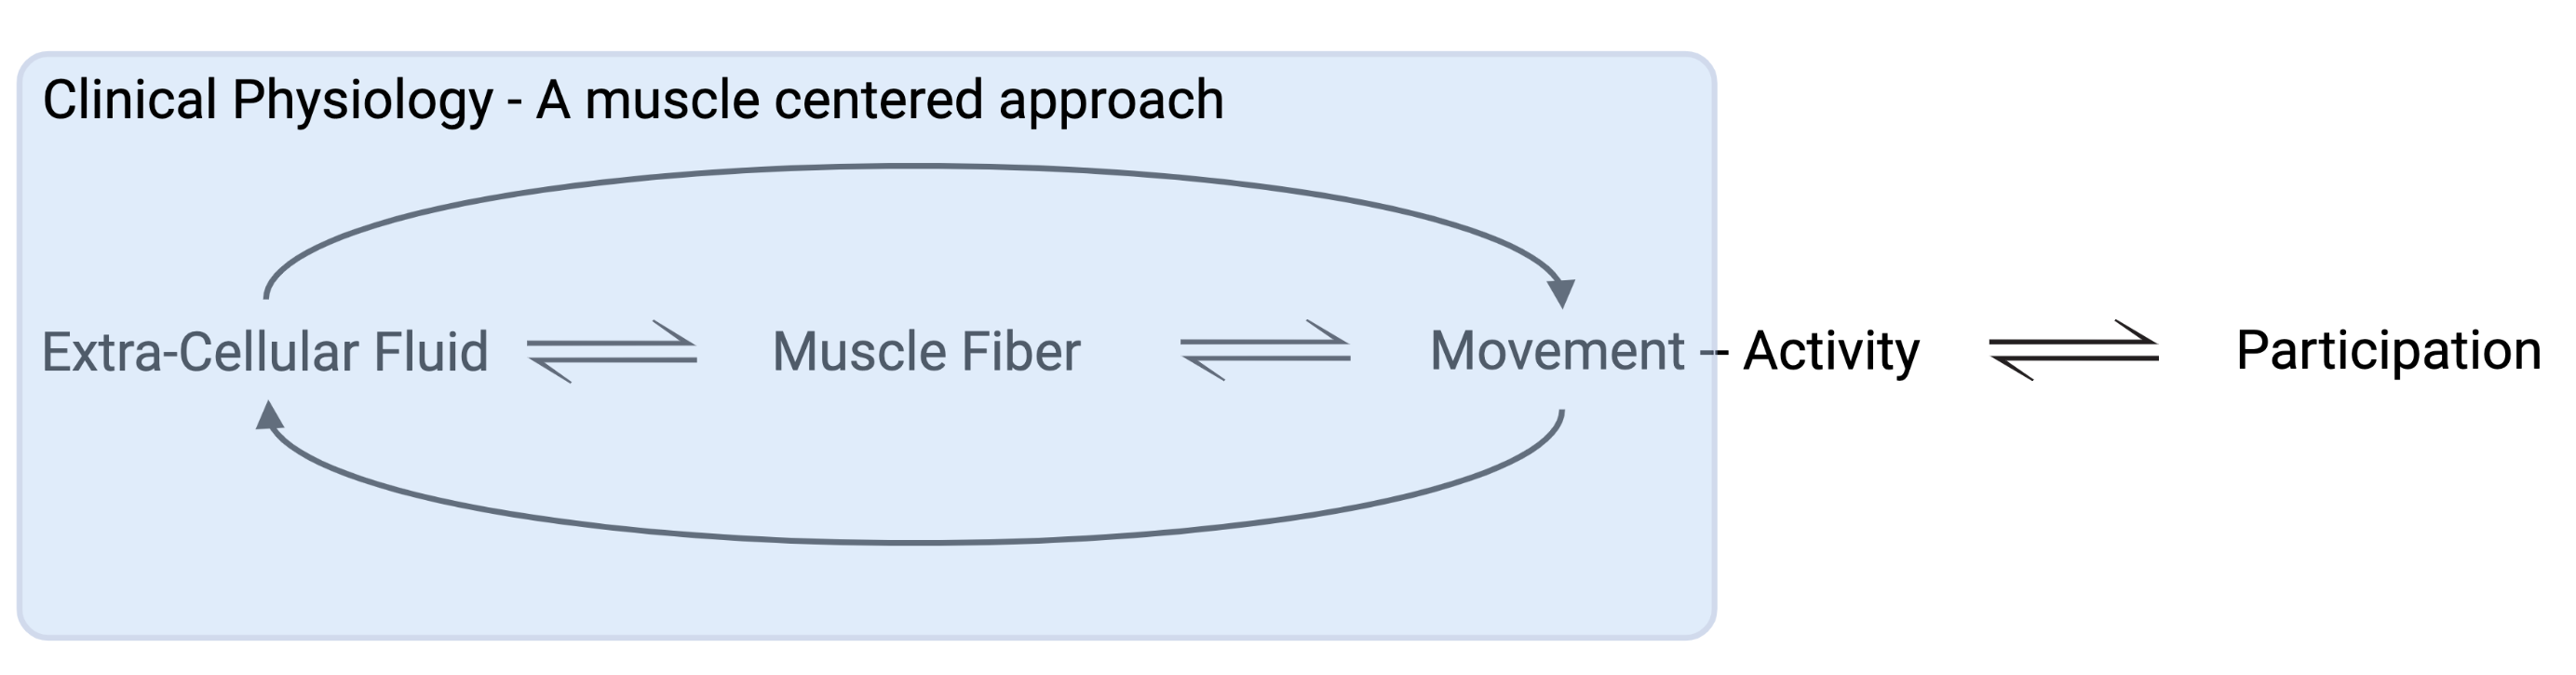
\includegraphics[width=1\linewidth]{./figure/muscle_centered_approach_icf.png}
    \caption{Muscle centered approach overlap with the ICF) \footnotesize{(Created with BioRender.com)}}
    \label{fig:muscle_centered_approach_icf}
\end{figure}

\section{Chapter Summary \& Next Steps}

Clinical physiology with a muscle centered approach for a physical therapist is based on the relationship between muscle fibers, movement and extra-cellular fluid. The muscle centered approach considers muscle fibers as crucially necessary, but not sufficient, causes of movement. Movement is a complex multi-system physiological function and capacity through its contribution to the ECF (Figure \ref{fig:muscle_centered_approach}). Movement is critical to the health and well being of the body given that movement is critical to the ECF, and the ECF is critical to all cells in the body. The muscle centered approach is a \textit{middle out} approach to understanding the complexity and hierarchy of physiology for the physical therapist as a movement specialist. By \textit{middle out} we refer to the entire approach as a model of clinical physiology that looks upward in scale (movement as a behavior within a culture) and looking downward in scale (to the genes).

\paragraph{Next Steps}
Part I is focused on Muscle Fidelity \& Efficacy, what it takes for muscle to attain, sustain and persevere in the act of tensioning. Part II is focused on Muscle Support, what it takes to support muscle fibers in the act of attaining, sustaining and persevering in the act of tensioning. Part III focuses on Muscle Integrity, how do muscle fibers persevere and maintain under steady state and variable conditions and in the face of threats to integrity (damage, injury and illness).  

\printbibliography[heading=subbibintoc]